% ==================================================
%  Capítulo 6 — Optimización y Diseño Inverso
% ==================================================
\section{Optimización y Diseño Inverso}\label{sec:optimizacion}

Esta sección describe la estrategia de optimización para resolver el problema inverso: encontrar la geometría de metalente que maximiza la calidad de enfoque. Al igual que el modelado (Sección~\ref{sec:modelado}), la estrategia evolucionó desde una búsqueda global libre hacia una búsqueda restringida al manifold de geometrías validadas, complementada con un refinamiento final por simulación directa.

% --------------------------------------------------
\subsection{Formulación del Problema}\label{subsec:formulacion}

El diseño inverso se formula como la maximización de la aptitud predicha por el surrogate, sujeta a las restricciones físicas del sistema:

\begin{equation}
    \mathbf{x}^* = \arg\max_{\mathbf{x} \in \mathcal{X}} \; \mathcal{F}(\mathbf{x}),
    \label{eq:optimization}
\end{equation}

\noindent donde $\mathbf{x} = [\text{widths}_{(101)},\; c_{2c}]$ es el vector de 102 dimensiones que define la geometría, $\mathcal{F}$ la función de aptitud derivada del surrogate, y $\mathcal{X}$ el espacio factible:

\begin{align}
    0.020 \leq w_i &\leq 0.300 \;\mu\text{m}, & &\forall\, i \in \{1,\ldots,101\}, \label{eq:c1} \\
    0.150 \leq c_{2c} &\leq 0.300 \;\mu\text{m}, & & \label{eq:c2} \\
    c_{2c} - \tfrac{1}{2}(w_i + w_{i+1}) &\geq 0.020 \;\mu\text{m}, & &\forall\, i, \label{eq:c3} \\
    0.1 \leq w_i / c_{2c} &\leq 0.5, & &\forall\, i. \label{eq:c4}
\end{align}

Las dos primeras restricciones, (\ref{eq:c1}) y (\ref{eq:c2}), fijan los rangos físicos de los anchos y de la separación centro a centro, el régimen sub-longitud de onda ya descrito en la Sección~\ref{subsec:variables}; (\ref{eq:c3}) garantiza una pared sólida de oro entre rendijas contiguas, y (\ref{eq:c4}) mantiene el factor de llenado en el régimen de resonancia óptima para la EOT. Toda geometría propuesta por el optimizador se repara por proyección al espacio factible.

% --------------------------------------------------
\subsection{Selección del Algoritmo: Algoritmo Genético}\label{subsec:seleccion_ga}

Se seleccionó un Algoritmo Genético (GA) por tres razones: (i)~el espacio de 102 dimensiones con restricciones no lineales es su nicho natural; (ii)~la aptitud se trata como una caja negra no diferenciable; y (iii)~la evaluación del surrogate en milisegundos hace viable operar poblaciones grandes sin costo significativo. El segundo punto merece justificación: aunque el MLP es diferenciable, el objetivo que guía la búsqueda no se evalúa sobre su salida cruda, sino que se construye \emph{post-procesándola}, se detecta el pico focal y se extraen descriptores del perfil de intensidad (Sección~\ref{subsec:manifold}), y exige proyectar cada candidato a un espacio factible con restricciones duras; ambas operaciones son no diferenciables. Y aunque se quisiera ascender el gradiente del surrogate directamente, ello conduciría a sus regiones de extrapolación, donde sobreestima (Sección~\ref{subsec:eval_surrogate}). El gradiente, por tanto, no es aprovechable y se opta por una metaheurística sin gradiente. La Optimización Bayesiana se descartó por la escalabilidad de los Procesos Gaussianos a 102 dimensiones ($\mathcal{O}(n^3)$).

Cada individuo codifica una metalente como un vector de 102 genes continuos. Los operadores son: selección por torneo (tamaño 5), cruzamiento SBX (\textit{Simulated Binary Crossover}~\cite{deb1995sbx}, $\eta = 15$, probabilidad $0.8$), mutación gaussiana (tasa $5\%$ por gen) con proyección al espacio factible, y elitismo (los 10 mejores pasan intactos). La población es de $250$--$500$ individuos y se ejecutan $80$--$200$ generaciones.

% --------------------------------------------------
\subsection{Primer Enfoque: Ciclo Activo y su Limitación}\label{subsec:ciclo_activo}

El planteamiento inicial integró el GA en un ciclo activo cerrado. En cada iteración se re-entrenaba el surrogate, se seleccionaban geometrías inciertas mediante \textit{Query by Committee} para simular por FDTD, se ejecutaba el GA con el surrogate actualizado, y se confirmaban sus mejores candidatos. Cada ciclo añadía $15$ simulaciones ($10$ de aprendizaje activo $+ 5$ del GA).

La confirmación FDTD reveló la limitación central: el GA, al optimizar sin restricción sobre todo el espacio, explotaba las debilidades del surrogate. Convergía rápidamente (en $9$--$14$ generaciones) a regiones saturadas del espacio, cerca del borde superior de $c_{2c}$ y de los anchos máximos permitidos por el factor de llenado, donde el surrogate predecía $R^2$ alto por no haber visto datos ahí, no por enfoque real. Los candidatos resultantes tenían $R^2$ predicho ${\sim}0.98$ pero $R^2$ real $\in [0.47, 0.54]$ (brecha media $+0.48$). La correlación global positiva del surrogate no bastaba: el optimizador encuentra los puntos donde el modelo falla.

\paragraph{Lección y re-enfoque.} Este primer enfoque no produjo diseños útiles, pero su utilidad reside en la lección metodológica que deja. Dejó dos lecciones que definieron todo lo posterior: (i)~una correlación global positiva del surrogate no garantiza nada, porque el optimizador busca los puntos donde el modelo falla; y (ii)~la libertad de búsqueda es contraproducente con un surrogate imperfecto. El re-enfoque, por tanto, abandona la búsqueda global y el ciclo activo, y los reemplaza por dos cambios concretos: (a)~restringir la búsqueda al manifold de geometrías validadas (Sección~\ref{subsec:manifold}) para impedir la extrapolación, y (b)~sustituir la función de aptitud por una combinación que siga discriminando dentro de ese manifold (Sección~\ref{subsubsec:combo}). Un refinamiento final por simulación directa (Sección~\ref{subsec:hill_climbing}) cierra la estrategia. Las siguientes secciones desarrollan cada pieza, todo lo descrito a partir de aquí pertenece ya al enfoque definitivo.

% --------------------------------------------------
\subsection{Diseño Inverso Restringido al Manifold}\label{subsec:manifold}

El re-enfoque parte de restringir el GA al manifold de geometrías validadas (concepto introducido en la Sección~\ref{subsec:diseno_inverso}). En lugar de buscar en todo $\mathcal{X}$, la población se inicializa y se mantiene en una caja $\ell_\infty$ de radio reducido alrededor de geometrías ya confirmadas como buenos enfocadores (semillas):

\begin{equation}
    \|\mathbf{x} - \mathbf{x}_{\text{seed}}\|_{\infty} \leq \delta, \qquad
    \delta \in \{20, 10, 5\}\;\text{nm}.
    \label{eq:manifold_box}
\end{equation}

Cada individuo se asocia a una semilla de origen; la reproducción ocurre dentro del mismo \textit{cluster} (sin cruzamiento entre cuencas distintas) y cada hijo se proyecta de vuelta a la caja. Por continuidad física, perturbaciones pequeñas ($\leq 20$~nm) de un enfocador conocido aumentan la probabilidad de permanecer en una región ópticamente plausible y reducen el riesgo de extrapolación del surrogate, aunque no garantizan estabilidad óptica. El radio $\delta$ se redujo progresivamente entre iteraciones (20~nm $\rightarrow$ 10~nm $\rightarrow$ 5~nm) para refinar la búsqueda. La Figura~\ref{fig:manifold_esquema} ilustra la idea: un optimizador libre escapa hacia las regiones de extrapolación donde el surrogate sobreestima, mientras que la caja $\ell_\infty(\delta)$ mantiene la búsqueda en el vecindario validado.

\begin{figure}[H]
    \centering
    \resizebox{0.85\textwidth}{!}{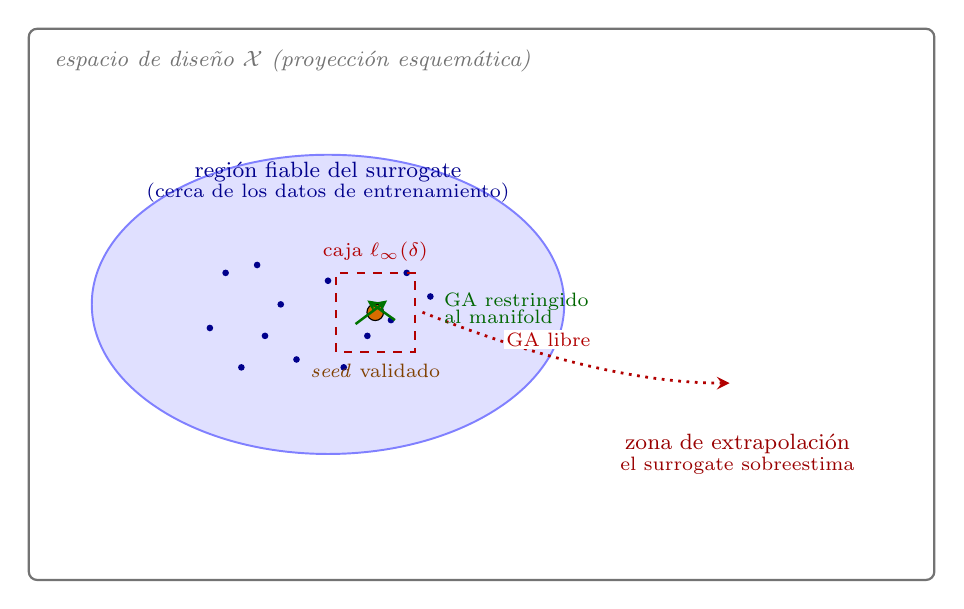
\begin{tikzpicture}[>=stealth, font=\small]

  % --- Espacio de diseño ---
  \draw[rounded corners=3pt, draw=black!55, line width=0.8pt] (0,0) rectangle (11.5,7);
  \node[anchor=north west, font=\footnotesize\itshape, text=black!55] at (0.2,6.85)
      {espacio de diseño $\mathcal{X}$ (proyección esquemática)};

  % --- Región fiable del surrogate (cerca de los datos) ---
  \fill[blue!12] (3.8,3.5) ellipse (3.0 and 1.9);
  \draw[blue!50, line width=0.7pt] (3.8,3.5) ellipse (3.0 and 1.9);
  \node[blue!55!black, font=\footnotesize, align=center] at (3.8,5.05)
      {región fiable del surrogate\\[-2pt]{\scriptsize(cerca de los datos de entrenamiento)}};

  % --- Datos de entrenamiento ---
  \foreach \x/\y in {2.3/3.2,2.9/4.0,3.4/2.8,3.8/3.8,4.3/3.1,4.8/3.9,2.7/2.7,3.2/3.5,4.6/3.3,5.1/3.6,2.5/3.9,4.0/2.7,3.0/3.1}
     \fill[blue!55!black] (\x,\y) circle (1.2pt);

  % --- Zona de extrapolación ---
  \node[red!60!black, font=\footnotesize, align=center] at (9.0,1.6)
      {zona de extrapolación\\[-2pt]{\scriptsize el surrogate sobreestima}};

  % --- Seed validado + caja L-infinito ---
  \fill[orange!85!black] (4.4,3.4) circle (3pt);
  \draw[black] (4.4,3.4) circle (3pt);
  \draw[dashed, red!70!black, line width=0.8pt] (3.9,2.9) rectangle (4.9,3.9);
  \node[red!70!black, font=\scriptsize, anchor=south] at (4.4,3.92) {caja $\ell_\infty(\delta)$};
  \node[font=\scriptsize, anchor=north, text=orange!50!black] at (4.4,2.86) {\textit{seed} validado};

  % --- GA libre (malo): escapa hacia la extrapolación ---
  \draw[->, red!70!black, line width=1.0pt, dotted]
      (5.0,3.4) .. controls (7,2.6) and (8.2,2.5) .. (8.9,2.5);
  \node[red!70!black, font=\scriptsize, fill=white, inner sep=1pt] at (6.6,3.05) {GA libre};

  % --- GA restringido (bueno): se mantiene en la caja ---
  \draw[->, green!45!black, line width=0.9pt] (4.15,3.25) -- (4.55,3.55);
  \draw[->, green!45!black, line width=0.9pt] (4.65,3.3) -- (4.3,3.55);
  \node[green!40!black, font=\scriptsize, anchor=west, align=left] at (5.15,3.45)
      {GA restringido\\[-2pt]al manifold};

\end{tikzpicture}
}
    \caption{Restricción al manifold (esquemática). Las geometrías validadas (puntos) y su
    vecindario definen la región donde el surrogate es fiable; fuera de ella el modelo
    extrapola y sobreestima. Un GA libre (flecha roja punteada) deriva hacia esa zona y
    produce candidatos no fiables; el GA restringido mantiene la población dentro de la caja
    $\ell_\infty(\delta)$ alrededor de una semilla confirmada.}
    \label{fig:manifold_esquema}
\end{figure}

\subsubsection{Función de Aptitud Combinada}\label{subsubsec:combo}

El segundo pilar del re-enfoque atañe a \emph{qué} se optimiza. Una aptitud combinada es, como se anticipó en la Sección~\ref{subsec:diseno_inverso}, una función de aptitud que suma varios términos medibles en lugar de uno solo, y se vuelve necesaria aquí por la siguiente observación. Dentro del manifold, la cabeza $\hat{R}^2_{\text{pred}}$ del surrogate satura (varianza $<10^{-3}$) y deja de discriminar entre geometrías casi idénticas. Sin embargo, dos descriptores auxiliares derivados del campo predicho, es decir, el ancho a media altura (FWHM) del perfil de intensidad, que mide el tamaño del foco, y su concentración (cociente máximo/media), que mide cuán apuntado es, conservan poder discriminativo, con correlaciones $|{\sim}0.9|$ respecto al $R^2$ real. Se definió entonces la aptitud como:

\begin{equation}
    \mathcal{F}(\mathbf{x}) = \hat{R}^2_{\text{pred}}
    + \alpha\, z_{\text{conc}}(\mathbf{x}) - \beta\, z_{\text{fwhm}}(\mathbf{x}),
    \label{eq:combo_fitness}
\end{equation}

\noindent donde $z_{\text{conc}}$ y $z_{\text{fwhm}}$ son los $z$-scores de concentración y
FWHM calculados \emph{por generación} (adaptativos a la población actual). Los coeficientes
$\alpha = 0.098$ y $\beta = 0.108$ se calibraron por mínimos cuadrados ordinarios sobre las
geometrías confirmadas de una iteración previa ($R^2_{\text{OLS}} = 0.85$). El término
$\hat{R}^2_{\text{pred}}$ ancla la aptitud hacia la zona globalmente alta, mientras que los
términos auxiliares discriminan entre candidatos cercanos cuando el escalar satura.

Para preservar diversidad, la selección de los candidatos finales se diversifica por
\textit{cluster} (un número fijo por cada semilla), evitando que todos converjan a una
sola cuenca.

% --------------------------------------------------
\subsection{Refinamiento Final: Hill-Climbing por Simulación Directa}\label{subsec:hill_climbing}

Tras varias iteraciones del GA restringido (descritas en la
Sección~\ref{sec:resultados}), se constató que el surrogate ya no aportaba dirección de mejora dentro de las cuencas: las geometrías de alta calidad conocidas estaban en óptimos locales estrechos. El paso final prescindió del surrogate y empleó hill-climbing por simulación FDTD directa (búsqueda local en el sentido de la Sección~\ref{subsec:diseno_inverso}): alrededor de cada cuenca de interés se generaron $50$ perturbaciones gaussianas ($\sigma = 5$~nm) de la mejor geometría conocida, validando cada una por FDTD. Todas las perturbaciones respetan las restricciones físicas mediante recorte al manifold válido.

Este procedimiento cumple un doble propósito: refinar la mejor geometría sin el sesgo del surrogate, y caracterizar la robustez local de cada cuenca, es decir, qué tan sensible es el $R^2$ a perturbaciones del orden de las tolerancias de fabricación. Los resultados de este análisis, que revelaron diferencias cualitativas entre cuencas, se presentan en la Sección~\ref{sec:resultados}.
